\setcounter{subsection}{22-1}
\subsection{The Quotient Topology}

% Useful macros for this section
\def\ivp{\inv{p}}
\newcommand\ivpss[1]{\ivp\parens{\braces{#1}}}

\exercise{1}{
  Check the details of Example~3.
}
\sol{
  Recall that Example~22.3 includes a function $p: \reals \to A$ where $A = \braces{a,b,c}$ is a three-point set.
  The function is defined by
  \gath{
    p(x) = \begin{cases}
      a & x > 0 \\
      b & x < 0 \\
      c & x = 0 \,.
    \end{cases}
  }
  We are then asked to verify that the quotient topology on $A$ induced by $p$ is that indicated by the following diagram:
  \begin{center}
    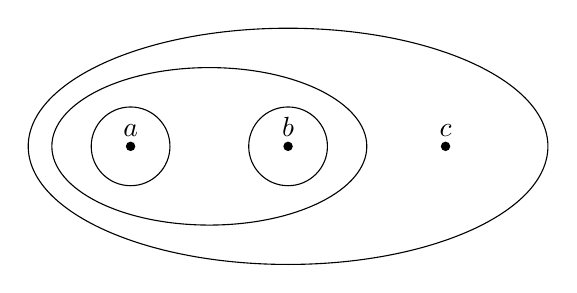
\begin{tikzpicture}
      % Points
      \fill (-2,0) circle (0.06);
      \fill (0,0) circle (0.06);
      \fill (2,0) circle (0.06);

      % Point labels
      \node [above] at (-2,0) {$a$};
      \node [above] at (0,0) {$b$};
      \node [above] at (2,0) {$c$};

      % Single point subsets
      \draw (-2,0) circle (0.5);
      \draw (0,0) circle (0.5);

      % Two-point subsets and full set
      \draw (-1, 0) circle (2 and 1);
      \draw (0, 0) circle (3.3 and 1.5);
    \end{tikzpicture}
  \end{center}
  \qproof{
    Clearly the diagram illustrates the topology $\cT = \braces{\es, \braces{a}, \braces{b}, \braces{a,b}, A}$ on $A$.
    We also note that $p$ is surjective, and that $\cT$ is the unique topology such that $p$ is a quotient map.
    First, obviously $\es$ and $A$ must be open in the quotient topology $\cT$ since it is a topology.
    Then, clearly the following sets
    \ali{
      \ivpss{a} &= (0, \infty) \\
      \ivpss{b} &= (-\infty, 0) \\
      \ivpss{a,b} &= (0, \infty) \cup (-\infty, 0)
    }
    are all open in $\reals$ so that $\braces{a}$, $\braces{b}$, and $\braces{a,b}$ should be open in the quotient topology since $p$ is a quotient map.
    On the contrary, the sets
    \ali{
      \ivpss{c} &= \braces{0} \\
      \ivpss{a,c} &= \clop{0, \infty} \\
      \ivpss{b,c} &= \opcl{-\infty, 0}
    }
    are all clearly not open in $\reals$ (in fact they are all closed) so that $\braces{c}$, $\braces{a,c}$ and $\braces{b,c}$ should not be open in the quotient topology.
    As we have considered all eight of the possible subsets of $A$, this shows the desired result.
  }
}

\exercise{2}{
  \eparts{
  \item Let $p: X \to Y$ be a continuous map.
    Show that if there is a continuous map $f: Y \to X$ such that $p \circ f$ equals the identity map of $Y$, then $p$ is a quotient map.
  \item If $A \ss X$, a \boldit{retraction} of $X$ onto $A$ is a continuous map $r: X \to A$ such that $r(a) = a$ for each $a \in A$.
    Show that a retraction is a quotient map.
  }
}
\sol{
  (a)
  \qproof{
    First, $f$ is a right inverse for $p$ by definition so that $p$ is surjective by Exercise~2.5 part (a).
    Suppose that $U$ is a subset of $Y$.
    If $U$ is open in $Y$ then $\ivp(U)$ is open in $X$ since $p$ is continuous.
    So suppose that $V = \ivp(U)$ is open in $X$.
    Since we have $p \circ f = i_Y$ is bijective and $i_Y = \inv{i_Y}$, it follows from Exercise~2.4 part~(a) that
    \gath{
      U = i_Y(U) = \inv{i_Y}(U) = \inv{(p \circ f)}(U) = \ivf(\ivp(U)) = \ivf(V) \,.
    }
    Then, since $V$ is open in $X$, we have that $\ivf(V) = U$ is open in $Y$ since $f$ is continuous.
    This shows that $p$ is a quotient map by definition.
  }

  (b)
  \qproof{
    Suppose $X$ is a topological space, $A \ss X$, and $r: X \to A$ is a retraction.
    Let $f: A \to X$ be defined by $f(a) = a$ for all $a \in A$, i.e. $f$ is the identity function on $A$ with the range expanded to $X$.
    Now, $i_A$ is continuous (in fact it is a homeomorphism) by Exercise~18.3 so that $f$ is also continuous by Theorem~18.2 part~(e) since it is just $i_A$ with an expanded range.
    Then for any $a \in A$ we have that
    \gath{
      (p \circ f)(a) = p(f(a)) = p(a) = a
    }
    since $p$ is a retraction.
    Thus $p \circ f = i_A$, which shows that $p$ is a quotient map by what was shown in part~(a).
  }
}

\def\realss{\reals \times \reals}
\exercise{3}{
  Let $\pi_1: \realss \to \reals$ be projection on the first coordinate.
  Let $A$ be the subspace of $\realss$ consisting of all points $x \times y$ for which either $x \geq 0$ or $y = 0$ (or both); let $q: A \to \reals$ be obtained by restricting $\pi_1$.
  Show that $q$ is a quotient map that is neither open nor closed.
}
\sol{
  \qproof{
    First consider any $x \in \reals$ and the point $x \times 0$, which is clearly in $A$ by definition.
    Then we have $q(x \times 0) = \pi_1(x \times 0) = x$, which shows that $q$ is surjective since $x$ was arbitrary.
    Now, since we know that $\pi_1$ is continuous, its restriction $q$ is also continuous by Theorem~18.2 part~(d).
    So, suppose that $U$ is a saturated open set of $A$ so that $U = \inv{q}(V)$ for some subset $V \ss \reals$.
  }
}
